\documentclass{article}
% Editable hybrid-model scaffold: neural architecture and results are proposed.
\IfFileExists{iclr2025_conference.sty}{\usepackage{iclr2025_conference,times}}{
  \usepackage[margin=1in]{geometry}\usepackage{times}
  \usepackage[round,authoryear]{natbib}}
\usepackage[T1]{fontenc}
\usepackage[utf8]{inputenc}
\usepackage{amsmath,amssymb,booktabs,microtype,xcolor}
\usepackage{tikz}
\usetikzlibrary{arrows.meta,positioning}
\usepackage{hyperref,url}
\newcommand{\model}{\textsc{DiffMars}}
\newcommand{\pending}[1]{\textcolor{blue!65!black}{[To complete: #1]}}
\newcommand{\resultpending}{\textit{Pending}}
\title{DiffMars: A Differentiable Mars General Circulation Model\\
with Constrained Neural Mixing}
\author{Anonymous authors}
\begin{document}
\maketitle

\begin{abstract}
Learning atmospheric models for Mars requires both a simulator whose coupled
trajectories can be differentiated and a learning interface that retains
physical structure. We develop \model, a differentiable Mars general
circulation model, and use its gradients for two linked tasks: inference of
interpretable physical parameters and end-to-end learning of a constrained
neural closure. In the completed T21/12-level simulator, gradient-based
optimization recovers one and three physical parameters from synthetic
trajectories: L-BFGS-B passes all six multistart fits under a 100-evaluation
ceiling. Thirteen paired physics and parameter experiments identify
boundary-layer mixing as an influential forecast pathway; removing it produces
the largest wind response among the tested process removals, while halving the
timestep changes atmospheric temperature by only 0.0042 K RMSE over 44,400 s.
Motivated by this sensitivity, a shared multilayer perceptron predicts bounded
corrections to momentum diffusivity and turbulent Prandtl number inside the
existing conservative column solver, initializing exactly at the physical
closure. The proposed objective differentiates multistep temperature and wind
errors against subdaily MACDA reanalysis through the coupled atmosphere. Thus
differentiability is both a verified capability of the physical model and the
mechanism that connects the neural parameterization to forecast error.
\pending{Insert held-out neural forecast improvement, multiseed uncertainty,
and neural/constant runtime ratio after matched evaluation. Couple the marginal
accuracy gain over learned constants to its runtime cost; report a null or
negative result explicitly if state dependence provides no detectable benefit.}
\end{abstract}

\section{Introduction}
Planetary atmospheric prediction couples a data problem to a physical modeling
problem. Observations sample selected locations, seasons, and atmospheric
properties, while a simulator must evolve a complete three-dimensional state.
Making that simulator differentiable adds a third requirement: sensitivities
must propagate through resolved dynamics, column physics, and interacting
surface reservoirs over a rollout. Those trajectory gradients provide a common
interface for calibrating interpretable parameters and training learned
components against forecast targets.
On Mars, radiation, surface heat storage, and turbulent exchange jointly
determine temperature and wind profiles in a thin atmosphere. This coupling
creates compensating errors: stronger radiative heating can offset excessive
heat removal, while stronger momentum mixing can reduce a wind bias caused by
an incorrect heating profile. A lower forecast error can therefore accompany
an incorrect allocation of tendencies among processes. Sparse planetary
observations make that ambiguity particularly consequential. We use it to
motivate a restricted learning interface: adjust the strength of an existing
transport mechanism while retaining its exchange structure and reservoirs.

Established Mars general circulation models combine dynamics with radiation,
surface thermodynamics, aerosols, and volatile exchange
\citep{forget1999improved,haberle2019ames}. Reanalyses combine physical
models with assimilated observations to produce temporally organized global
states. MACDA v2.0 and its ARCO distribution provide temperature, wind, pressure,
surface, and dust fields spanning multiple Mars years
\citep{valeanu2026macda,bhattacharya2026arcomars}. These resources enable a
concrete learning problem: optimize a parameterization through a coupled
rollout and evaluate its forecast trajectories in withheld years.

Hybrid general circulation models provide the computational precedent.
NeuralGCM couples differentiable atmospheric dynamics to learned
parameterizations and trains the coupled model using weather trajectories
\citep{kochkov2024neuralgcm}. Learned subgrid parameterizations also motivate
evaluation inside a prognostic model \citep{yuval2020stable}. Our architectural
choice is more specific than replacing physical tendencies with a neural
parameterization: the network predicts two bounded multipliers per vertical
interface, and a fixed conservative solver converts the resulting coefficients
into temperature and momentum tendencies. Learning can vary exchange strength,
but cannot introduce an independent heating or acceleration term through this
interface. This restriction limits the available corrections but does not identify their
physical cause: mixing can still compensate for errors in radiation, dust,
surface forcing, or initialization. We therefore interpret fitted coefficients
as forecast corrections conditional on this fixed backbone, rather than as
recovered physical transport coefficients.

We choose boundary-layer mixing because it connects surface forcing to both
forecast targets, temperature and wind, through uncertain subgrid transport.
Our baseline prescribes a mixing depth and stability-dependent coefficients;
these provide a concrete, low-dimensional interface for state-dependent
learning. The completed paired ablations supply an empirical selection
criterion: removing mixing produces the largest wind response among the tested
process removals, with zonal and meridional differences of 1.66 and 1.57 m/s
RMSE over 44,400 s. Halving the timestep changes each wind component by less
than 0.01 m/s over the same interval. These sensitivities identify mixing as
an influential intervention point; matched held-out forecasts will test
whether changing its coefficients improves prediction.

We ask two connected questions: \emph{can a Mars GCM expose useful gradients
through coupled physical trajectories, and can those same gradients train a
bounded, state-dependent mixing closure that improves temperature and wind
forecasts relative to fixed and scalar-calibrated closures?} The first question
establishes differentiability through synthetic parameter recovery. The second
uses boundary-layer mixing as a focused neural-learning problem because it
couples surface forcing to both forecast targets. The neural module adjusts
momentum diffusivity and the relative efficiency of heat transport while
preserving positive coefficients; its initialization recovers the existing
physical model. The physical closure is therefore both the baseline and the
starting point of end-to-end learning. We organize the paper around three
contributions:
\begin{enumerate}
\item A differentiable Mars GCM with explicit atmosphere, surface, regolith,
and frost reservoirs, together with verified trajectory gradients and
gradient-based recovery of physical parameters.
\item Controlled process ablations that identify boundary-layer mixing as an
influential temperature--wind pathway and motivate the learned intervention.
\item A proposed coefficient-learning architecture with two bounded,
identity-initialized outputs per interface, retaining the physical solver's
layer-mass weighting, exchange support, and kinetic-energy return, plus a
subdaily reanalysis protocol comparing physical, scalar-calibrated, and neural
closures across forecast horizons and seasons.
\end{enumerate}
\pending{Replace proposed-method contribution statements with measured neural
findings when the experiments are complete.}

\section{Background and Related Work}
\subsection{Mars simulation and reference data}
The LMD and NASA Ames Mars GCMs establish detailed treatments of the Martian
atmosphere and its interaction with the surface
\citep{forget1999improved,haberle2019ames}. In \model, seasonal dust interacts
with radiation, while surface frost exchanges mass and latent heat with the
atmosphere. Boundary-layer mixing connects surface influences to circulation.
These processes act on overlapping observables: temperature responds to both
radiative heating and heat redistribution, while winds respond to thermal
gradients, surface drag, and momentum transport. Our design holds the other
operators fixed within each matched learning experiment and exposes only the
mixing coefficients to the network.

MACDA v2.0 assimilates spacecraft observations to construct atmospheric and
surface fields \citep{valeanu2026macda}. ARCO-MACDA distributes those fields
in a chunked cloud-accessible format \citep{bhattacharya2026arcomars}.
MACDA is itself a model--assimilation product rather than direct observation.
We use reanalysis states as forecast targets and static topography and surface
maps as boundary inputs, and separate training and evaluation by Mars year.

\subsection{Differentiable and hybrid atmospheric models}
NeuralGCM combines differentiable spectral dynamics with neural
parameterizations that supply tendencies to the atmospheric evolution
\citep{kochkov2024neuralgcm}. \model{} uses the Dinosaur
spectral core associated with this modeling ecosystem.\footnote{
Dinosaur software: \url{https://github.com/neuralgcm/dinosaur};
the completed GPU experiments record version 1.3.6.}
Both approaches differentiate through coupled rollouts. In \model{}, this is a
primary model capability rather than only an implementation detail of neural
training: a single differentiable transition supports physical parameter
inference, sensitivity analysis, and optimization of learned closure
parameters. Synthetic recovery tests the first use before the same gradient
path is applied to the neural closure. The proposed architectural distinction
is the network's output and its route into the equations: \model{} predicts
multipliers of momentum diffusivity and turbulent Prandtl number, rather than a
vector of learned physical tendencies.
Each multiplier is restricted to a factor of two around the physical closure,
and zero output recovers that closure exactly. The unchanged implicit solver
then determines all associated mixing tendencies and dissipative heating.
The contribution under test is this restricted hypothesis class for Mars
trajectory learning, evaluated against both the original closure and
state-independent scalar calibration.

\subsection{Learning constrained subgrid transport}
A learned parameterization affects the evolving atmosphere, making coupled
trajectory evaluation essential \citep{yuval2020stable}.
In our proposed model, adjacent-layer exchange retains the same layer-mass
weights, positive coefficients, prescribed vertical support, and
kinetic-energy-to-heat calculation as the physical baseline. Consequently,
the network can redistribute properties through the existing operator rather
than supply arbitrary per-layer source terms. Regularization toward unit
multipliers further favors the baseline when the trajectory data provide
little evidence for a correction.

This yields a testable separation between parameter tuning and learned
state dependence. Constant multipliers test whether an overall change in
mixing strength is sufficient; the shared MLP tests whether conditioning on
stability, shear, and the column state improves withheld trajectories.
Momentum-only and Prandtl-only variants identify which coefficient changes
account for any improvement. Thus the evaluation examines the proposed
learning interface itself, rather than attributing a forecast gain solely
to adding a neural network.

\section{Method}
\subsection{Completed differentiable physical backbone}
Let \(x\) denote atmospheric state, \(s\) surface and subsurface reservoirs,
and \(b\) fixed boundary properties. The coupled model evolves
\begin{equation}
\frac{d}{dt}\begin{bmatrix}x\\s\end{bmatrix}
=\mathcal D(x;b)+\mathcal P_\phi(x,s,b,t).
\end{equation}
Atmospheric variables comprise spectral vorticity, divergence, temperature
variation, and log surface pressure. Additional states include surface and
soil temperatures and surface CO$_2$ frost. The calibrated physical parameters
are CO$_2$ and dust longwave opacity scales and a surface-exchange multiplier.

Completed experiments use T21 resolution, a \(64\times32\)
(longitude \(\times\) latitude) horizontal grid,
12 sigma levels, and IMEX-RK-SIL3 with a 300 s timestep. Coupled physics includes
diurnal and eccentric-orbit forcing, Ames-derived correlated-\(k\) CO$_2$
radiation, prescribed seasonal dust, MOLA topography, TES surface properties,
regolith conduction, surface drag and sensible heat exchange, vertical mixing,
dry convection, and surface CO$_2$ exchange. A global pressure projection
maintains atmosphere-plus-frost mass accounting.

The complete timestep is implemented as a differentiable map
\begin{equation}
(x_{n+1},s_{n+1})=F_{\phi,\theta}(x_n,s_n;b,t_n),
\end{equation}
where \(\phi\) denotes physical parameters and \(\theta\) denotes neural
closure parameters. Automatic differentiation composes this map over multiple
steps, so a trajectory loss supplies gradients with respect to either parameter
set. We test gradients operationally through bounded parameter recovery rather
than equating software-level differentiability with useful inference. The
recovery experiment establishes a smooth, informative path for the tested
horizons and parameters; it does not imply that every switch, limiter, or
season-long trajectory is smooth or identifiable.

\subsection{Completed physical mixing closure}
At interface height \(z_k\), the baseline diffusivity is
\begin{equation}
K_k=\kappa_{\mathrm{vK}}u_*\max(z_k,1\,\mathrm{m})
[\max(0,1-z_k/h)]^2 f_{\mathrm{stab}}(\mathrm{Ri}_k),
\end{equation}
where \(u_*\) is friction velocity, \(h=5000\) m is prescribed mixing height,
and \(f_{\mathrm{stab}}\) smoothly adjusts mixing using a gradient Richardson
number. Potential temperature supplies the stability diagnostic; heights
are estimated from sigma coordinates using a reference scale height.

Momentum exchange uses a smoothly capped rate derived from
\(K_k/\Delta z_k^2\), capped near \(1/1800\ \mathrm{s}^{-1}\).
The heat rate is the momentum rate divided by a stability-dependent turbulent
Prandtl number. The solver acts on temperature variation and horizontal winds
with layer-mass weights. A backward-Euler tridiagonal solve uses a fixed
1800 s closure interval and returns tendencies to the outer integrator.
Resolved kinetic energy dissipated by mixing is returned as atmospheric heat.

\subsection{Proposed bounded neural mixing}
At each interface, form a 13-component feature vector
\begin{equation}
q_k=(T_k,T_{k+1},u_k,u_{k+1},v_k,v_{k+1},
\sigma_k,\sigma_{k+1},z_k,\mathrm{Ri}_k,u_*,T_s,p_s).
\end{equation}
Standardize continuous features using training-only statistics with a positive
scale floor. A shared MLP with two 32-unit hidden layers and SiLU activations
produces \(a_{K,k}\) and \(a_{\mathrm{Pr},k}\). Including biases, the network
has 1,570 trainable parameters. Define
\begin{equation}
m(a)=\exp[(\log2)\tanh(a)],\quad
K_k^\theta=K_km(a_{K,k}),\quad
\mathrm{Pr}_k^\theta=\mathrm{Pr}_km(a_{\mathrm{Pr},k}).
\label{eq:closure}
\end{equation}
Multipliers lie between \(1/2\) and \(2\). Zero-initialize the final layer,
with nonzero hidden-layer initialization, to start exactly at the physical
closure. This is a stability-motivated design choice, not a claim of architectural
novelty. Coupled learned parameterizations have established the importance of
online stability \citep{yuval2020stable}; positivity and identity initialization
alone do not guarantee stability of the full coupled rollout.
The bounded mapping also introduces a sensitivity tradeoff:
\(d\log m/da=(\log 2)\operatorname{sech}^2(a)\) tends to zero near
either bound. Small responses to logit perturbations must therefore be
interpreted alongside saturation and effective exchange rates.
Apply the diffusivity correction before the existing momentum-rate
cap; divide the capped rate by the corrected Prandtl number for heat transport.

Retain the column solver, kinetic-energy return, and spectral transforms.
The multiplicative design retains the baseline mixing support, including
zero diffusivity above its prescribed depth. Radiation, resolved dynamics,
surface exchange, regolith, convection, and CO$_2$ exchange remain physical.

\begin{figure}[t]
\centering
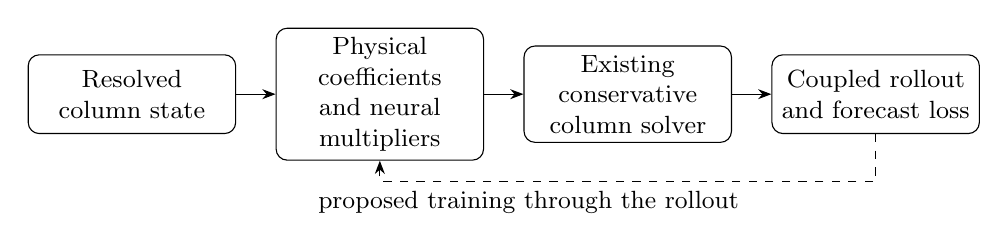
\begin{tikzpicture}[node distance=5mm,
box/.style={draw,rounded corners,align=center,font=\small,
text width=2.4cm,minimum height=10mm},>=Stealth]
\node[box] (state) {Resolved\\column state};
\node[box,right=of state] (coeff) {Physical coefficients\\and neural multipliers};
\node[box,right=of coeff] (solve) {Existing conservative\\column solver};
\node[box,right=of solve] (rollout) {Coupled rollout\\and forecast loss};
\draw[->] (state)--(coeff);
\draw[->] (coeff)--(solve);
\draw[->] (solve)--(rollout);
\draw[->,dashed] (rollout.south)--++(0,-0.6)-|
node[pos=0.35,below,font=\small]{proposed training through the rollout}
(coeff.south);
\end{tikzpicture}
\caption{Proposed hybrid architecture. Learning adjusts exchange coefficients;
the physical solver computes tendencies.}
\end{figure}

\subsection{Proposed trajectory training}
For forecast times \(\tau\), fields \(c\in\{T,u,v\}\), cells \(i\), and layers
\(k\), define
\begin{equation}
\mathcal L(\theta)=\frac{1}{3|\mathcal T|}
\sum_{\tau,c,k,i}w_i\Delta\sigma_k
\left(\frac{\hat y^\theta_{\tau,c,k,i}-y_{\tau,c,k,i}}{s_c}\right)^2
+\lambda\,\mathbb E[(\log m_K)^2+(\log m_{\mathrm{Pr}})^2].
\end{equation}
Horizontal quadrature weights sum to one, \(\Delta\sigma_k\) weights layer
mass, and \(s_c\) is a training-only field scale. Regularization favors the
physical closure unless trajectory fitting supports a correction. Physical
parameters remain fixed and shared across matched neural comparisons.

Train using reverse-mode differentiation through short rollouts, with
checkpointing as required. The completed small-parameter recovery experiment
instead uses forward-mode tangents.
\pending{Specify optimizer, learning rate, normalization floors, regularization,
batch size, forecast horizons, gradient clipping, seeds, training budget,
and validation checkpoint selection.}

\section{Data and Experimental Setup}
\subsection{MACDA preprocessing and splits}
The verified ARCO-MACDA schema contains 96,480 states, 35 sigma levels, a
\(36\times72\) grid, and 12 snapshots per sol. Fields include atmospheric
temperature and winds, surface pressure and temperature, dust, and CO$_2$ ice.
The \texttt{swflux} and \texttt{lwflux} variables are downward surface shortwave
and longwave fluxes. Cite both the original MACDA v2.0 dataset and its ARCO
conversion \citep{valeanu2026macda,bhattacharya2026arcomars}.

Completed preprocessing streams bounded chunks, forms daily means, interpolates
to the model grid, and records hashes and finite-value checks. The proposed
neural pipeline retains native subdaily timestamps and contiguous sequences.
Validate units, gaps, sigma orientation, and periodic longitude mapping.
Represent observation times explicitly rather than silently rounding them to
300 s; any terminal fractional step retains fixed physical closure intervals.

The neural study will use the documented dataset split: MY24--27 and MY29--31
for training; MY32--33 for validation; MY34--35 for testing; MY28 for separate
dust-storm evaluation reported in the main text alongside MY34--35, rather than
pooled into a single headline score. Year labels alone do not define storm
regimes: classify windows using documented dust loading and seasonal metadata,
including storm episodes within the test years. Report each regime separately,
its sample count, and the dust forcing supplied to the model. Exclude the partial MY36 tail. Windows remain within
their assigned years and normalization uses training data only.
Existing physical calibration and synthetic recovery retain their own
experiment-specific configurations.

\subsection{Initialization and comparisons}
Initialize each model from the same regridded atmospheric state and use common
boundary maps, orbital alignment, and dust forcing. Convert CO$_2$ ice mass
per area consistently to the pressure-equivalent frost reservoir.
\pending{Specify and test soil-state initialization, spinup, pressure/topography
adjustments, and exact time/solar-longitude alignment.}
Future atmospheric reference states enter the loss only. Record whether dust
is climatological or reference-conditioned.

Compare unchanged physics, scalar-calibrated physics, and learned mixing.
Fit the scalar and neural baselines on training years using common targets.
Here scalar calibration means exactly two learned, state-independent logits
passed through Eq.~\ref{eq:closure}, rather than calibration of unrelated
physical parameters. Match bounds, identity initialization, loss,
regularization, training windows, forecast horizon, optimizer budget, and
validation selection to the MLP. First run a separate 200-update constant
baseline with validation every 50 updates as a screening comparison; this
short run does not replace the multiseed held-out evaluation. Retain the
bounded-MLP checkpoint and freeze its bounds and learning rate for this test.
Architecture ablations compare momentum-only, Prandtl-only, and joint
corrections under the same protocol.

Separately compare the current whole-atmosphere warmup with soil warmup
followed by resetting the atmosphere to the MACDA state at forecast start.
Specify which surface, frost, and soil reservoirs are retained and recheck
pressure and mass consistency after the reset. Use only information available
at or before forecast start. Cross initialization with physical, constant,
and neural closures using matched windows and retraining under each protocol;
report initial-state mismatch and subsequent forecast errors. Select the
initialization protocol on validation data before final testing.

\subsection{Metrics and evaluation}
Measure area- and layer-mass-weighted temperature and wind RMSE by lead time,
season, latitude, and height. Report surface pressure and temperature,
atmosphere-plus-frost mass drift, extrema, and rollout completion. Evaluate
five paired training seeds for the constant and neural models on identical
forecast windows. Define the primary comparison as neural minus constant
held-out loss, with field-specific RMSE differences as secondary outcomes.
Use a paired block bootstrap with 10,000 resamples: resample common temporal
blocks jointly across models and paired seed indices, recomputing weighted
RMSE from squared errors in each resample. Set block duration from validation
error autocorrelation, keeping overlapping windows together; grid cells and
lead times are not independent replicates. Report 95\% confidence intervals,
per-seed differences, block counts, and year/season/storm breakdowns. With
few held-out years, these intervals describe the sampled windows and training
variability, not uncertainty over all Mars climates. An interval containing
zero is inconclusive; it does not establish equivalence.

Measure synchronized post-compilation runtime on identical hardware,
resolution, timestep, precision, batch size, and output cadence. Report neural
slowdown relative to both physical and constant closures, compilation time,
peak device memory, training cost, and end-to-end forecast latency including
initialization and I/O. Use repeated matched measurements and report their
spread. Separate inference cost from gradient computation; do not infer
compiler or fusion overhead from parameter count alone.
\pending{Freeze lead times, window sampling, bootstrap block duration,
practically meaningful improvement threshold, and physical diagnostic
acceptance ranges before neural test-set evaluation. The five-seed and
bootstrap protocol above is planned, not a completed measurement.}

\section{Results}
\subsection{Completed gradient-based parameter recovery}
Noise-free targets are generated by the same simulator with CO$_2$ opacity,
dust opacity, and surface-exchange parameters \((0.6,0.8,1.4)\).
Training times are 6,000, 12,000, and 22,200 s; continuation samples at
30,000 and 44,400 s are evaluated afterward.
The completed objective uses horizontal area weighting and uniform layer
averaging; the proposed neural objective uses layer-mass weighting.

This experiment directly tests the simulator's differentiability claim:
gradients must pass through the coupled rollout and point to the known
parameters from multiple initial guesses. Both optimizers use bounded normalized coordinates, three starts, and a
100-oracle-evaluation ceiling per fit. Acceptance requires parameter errors
within 5\%, improved training and continuation losses, and passing gradient
checks.
\begin{table}[t]
\centering
\caption{Completed same-model synthetic recovery across three starts.
Calls are actual oracle evaluations.}
\begin{tabular}{llcc}
\toprule
Parameters & Optimizer & Successful fits & Calls per fit\\
\midrule
Surface exchange & L-BFGS-B & 3/3 & 9, 9, 8\\
Surface exchange & Powell & 3/3 & 100, 24, 24\\
All three & L-BFGS-B & 3/3 & 17, 20, 19\\
All three & Powell & 1/3 & 100, 100, 100\\
\bottomrule
\end{tabular}
\end{table}
The maximum relative parameter error across joint L-BFGS-B fits is
\(1.533\times10^{-6}\). This is parameter-recovery error, not adjoint or
gradient-check relative error. Same-model synthetic recovery verifies this
controlled inverse problem; it does not establish identifiability from
reanalysis under structural model error. Centered finite-difference checks use normalized
perturbations of \(10^{-3}\) and \(10^{-4}\).
\pending{Add the gradient-check plot from the verified recovery artifact.}

\subsection{Completed physics and timestep ablations}
All 13 sampled trajectories remain finite over 44,400 s from a common restart.
Table~\ref{tab:ablations} reports differences from full physics, averaged
over sampled times with horizontal area weights and equal layer weights.
The six additional cases perturb each of the three physical parameters by
factors of 0.8 and 1.2.
\begin{table}[t]
\centering
\caption{Completed paired sensitivities relative to full physics.}
\begin{tabular}{lrrr}
\toprule
Case & \(T\) RMSE (K) & \(u\) RMSE (m/s) & \(v\) RMSE (m/s)\\
\midrule
No boundary-layer mixing & 0.6729 & 1.6595 & 1.5682\\
No convection & 0.3201 & 0.4350 & 0.4099\\
No regolith & 0.7318 & 0.5998 & 0.6094\\
No CO$_2$ exchange & 0.1678 & 0.2789 & 0.2389\\
Weaker diffusion & 0.1854 & 0.6094 & 0.6209\\
Half timestep & 0.0042 & 0.0089 & 0.0098\\
\bottomrule
\end{tabular}
\label{tab:ablations}
\end{table}
Removing mixing produces the largest wind differences among these cases.
Halving the timestep costs 2.03 times the baseline execution time.
Maximum sampled relative atmosphere-plus-frost mass drift is
\(5.03\times10^{-12}\).
\pending{Insert verified year-long physical and neural diagnostics.}

\subsection{Completed computational measurements}
For a 74-step, 22,200-second trajectory, median synchronized execution over
three repeats is 2.125 s forward and 8.719 s for loss plus three forward
tangents, a ratio of 4.10. Recorded compilation times are 13.805 and 44.387 s.
Execution includes sampled field decoding and excludes input I/O, compilation,
and warmup. The recorded environment uses the JAX GPU backend and float64.
\pending{Add the original benchmark GPU model and measured peak device memory;
report neural timing separately.}

\subsection{Preliminary bounded-MLP diagnostic}
A preliminary checkpoint diagnostic reports a 0.276\% improvement in its
aggregate forecast objective. Across four examples at forecast-initial
interfaces, 78\% of sampled momentum multipliers are near the upper bound,
with mean multiplier 1.93. Momentum-logit perturbations produce little
forecast response, consistent with the bounded mapping's reduced sensitivity.
Prandtl corrections are not saturated and still affect forecasts. Wind
changes are mixed in the lower atmosphere: errors improve at
\(\sigma=0.875\) but worsen in the lowest layer, while upper-atmosphere
errors change little. This is evidence of momentum-correction saturation,
not a completely unresponsive network.

These small-sample, pre-rate-cap statistics neither establish held-out
improvement nor show that stronger mixing would generalize better. The
reported objective change is not a field-specific RMSE improvement. Useful
state dependence remains unestablished until the matched constant baseline
is evaluated. Upper-level insensitivity is also consistent with the fixed
vertical support of this closure.
\pending{Link the checkpoint and diagnostic artifact; specify the objective,
comparison baseline, sampled split, weighting, and numerical definition of
``near the bound.'' These figures are preliminary reported diagnostics and
must be verified before submission.}

\subsection{Neural experiments to complete}
Populate Table~\ref{tab:neural} using the matched held-out protocol. Add lead-time
curves, seasonal breakdowns, coefficient diagnostics, and architecture ablations.
\begin{table}[t]
\centering\small
\caption{Planned held-out comparison. Entries await matched evaluation;
report uncertainty across seeds and forecast windows.}
\begin{tabular}{lcccc}
\toprule
Model & \(T\) RMSE & \(u\) RMSE & \(v\) RMSE & Runtime\\
\midrule
Physical & \resultpending & \resultpending & \resultpending & \resultpending\\
Scalar-calibrated & \resultpending & \resultpending & \resultpending & \resultpending\\
Neural mixing & \resultpending & \resultpending & \resultpending & \resultpending\\
\bottomrule
\end{tabular}
\label{tab:neural}
\end{table}
Coefficient diagnostics are a main-text result required to interpret the
forecast comparison. Report multiplier distributions and saturation fractions
by height, season, latitude, stability, shear, and dust regime, at forecast
start and throughout rollouts. Distinguish inactive zero-diffusivity interfaces
from active interfaces and show both raw multipliers and realized post-cap
momentum/heat rates. Pair these with layerwise error changes and mixing,
radiative, and surface tendency budgets; physically plausible correlations
alone do not prove causal attribution.

Test compensation with a separate validation-selected sensitivity experiment
that varies dust/radiative forcing within documented plausible uncertainty,
keeping each forcing configuration identical across closure comparisons.
Report whether coefficient patterns and gains persist. If this experiment
is unavailable, explicitly retain the conditional forecast-correction claim
and the unresolved attribution limitation. Report MY28 and dust-stratified
test results with the same metrics and uncertainty as the headline result,
including degradations.

\subsection{Scope of the baseline comparison}
The prescribed-depth physical closure is a simplified baseline; improvements
over it do not establish superiority over LMD or Ames PBL treatments
\citep{forget1999improved,haberle2019ames}. A stronger comparison would implement
a documented established Mars mixing treatment in the same backbone, with
matched forcing, initialization, resolution, and tuning budget. Cross-model
published scores with different setups are not controlled closure comparisons.
\pending{Add the matched established-scheme baseline if feasible; otherwise
state explicitly that operational-scheme competitiveness is untested.}

\section{Conclusion}
We present \model{} as a differentiable Mars GCM and a constrained hybrid
model. Its coupled trajectory gradients recover physical parameters in a
controlled inverse problem, establishing differentiability as a measured result
and an inference tool. Paired ablations then identify boundary-layer mixing as
an influential pathway for both temperature and wind, motivating a neural
closure at that specific interface. The proposed network uses the same
trajectory gradients to learn bounded, state-dependent exchange coefficients
inside the conservative column solver. The next stage trains this closure on
subdaily MACDA trajectories and compares it with physical and
scalar-calibrated baselines. Together, parameter recovery and neural closure
learning form one story: differentiate through a structured Mars simulator,
then optimize either interpretable physical controls or a restricted learned
component without replacing the physical evolution.
\pending{Replace the final sentence with the measured held-out finding,
including storm performance and marginal runtime cost. Claim useful state
dependence only if the neural closure improves over matched learned constants
with uncertainty and practical effect size supporting that conclusion.
Otherwise state that this experiment has not demonstrated added value from
state dependence within the tested bounds, horizon, data, and backbone;
do not generalize a null result to all neural Mars closures.}

\bibliographystyle{plainnat}
\bibliography{references}
\appendix
\section{Implementation contract and remaining work}
The insertion point is coefficient calculation in
\texttt{pbl\_vertical\_diffusion\_tendencies}. Retain the weighted transport in
\texttt{\_implicit\_vertical\_diffusion\_tendency}.
Test identity initialization, bounded positive coefficients, finite gradients,
zero-mixing interfaces, and heat/momentum accounting.

The current PBL friction calculation passes reference air temperature to the
surface-exchange helper. Review this choice and freeze the baseline before
generating matched neural comparisons.

Remaining implementation steps:
\begin{enumerate}
\item Implement the shared MLP and parameter plumbing with baseline-identity tests.
\item Stage native-cadence sequences and implement matched initialization and
precise forecast-time alignment.
\item Validate reverse-mode gradients through short coupled trajectories.
\item Train scalar and neural closures, select checkpoints on validation years,
and evaluate fixed test windows across seeds.
\item Complete architecture ablations, longer rollouts, timing, and figures.
\end{enumerate}

\section{Reproducibility and evidence ledger}
Completed experiments record configuration, hashed inputs, source hashes,
and environments. Numerical results come from:
\begin{itemize}
\item Recovery directory: \path{outputs/paper-recovery-gpu/}.
Results: \texttt{parameter-recovery.csv}; detailed checks:
\texttt{recovery.json}.
\item \path{outputs/paper-ablations-gpu/ablations.csv}
and associated trajectories and diagnostic histories.
\item \path{outputs/paper-timing-gpu/timing.json}.
\item Data protocol: \path{docs/ideas/arco-macda-dataset-contract.md}.
\end{itemize}
The inspected ARCO-MACDA revision is
\texttt{65a0bebd804b9c240752277e83f5737d58c6ee9c}.
Archive selected windows, transformations, normalization statistics, splits,
and output hashes with each dataset. Retain attribution and license records
for both the original MACDA data and its CC BY 4.0 ARCO distribution.

\pending{Archive trained weights, configurations, seeds, hardware, selected
checkpoints, and evaluation commands. Update the conference style to the target
ICLR year's official template.}
\end{document}
